\section{Forced finance is reliable, and default redistributes the board}
\label{sec:default}

\subsection{All debt episodes}

A player whose debt exceeds its cash must raise money from a menu of mortgages and building sales, or declare bankruptcy. The cohort has \fact{debt.episodes} such debt episodes, \fact{debt.reasons.RENT} of them for rent. Players paid \fact{debt.paid} and were eliminated in \fact{debt.eliminated} (Figure~\ref{fig:debt}).

\begin{figure}[!htb]
\centering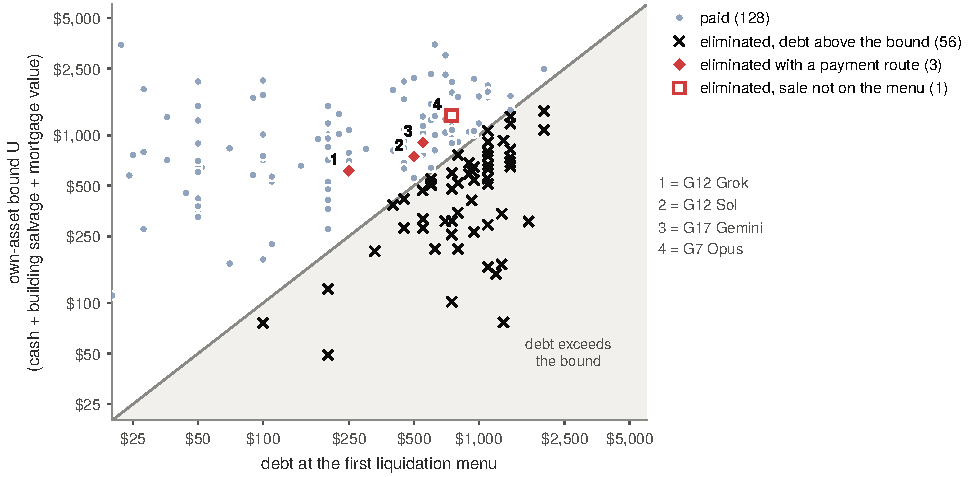
\includegraphics[width=0.92\linewidth]{fig_debt.pdf}
\caption{All \fact{debt.episodes} debt episodes at their first liquidation menu. The bound $U$ adds cash, the salvage value of every building and the mortgage value of every unmortgaged deed. A debt above $U$ cannot be paid from the player's own assets. Payment routes for the three numbered diamonds and the menu restriction for the square are inherited from earlier engine-executed checks.}
\label{fig:debt}
\end{figure}

For each episode we compute an own-asset bound $U$ at the first menu. It is the player's cash plus the salvage value of all its buildings plus the mortgage value of all its unmortgaged deeds. The bound ignores sale-order and bank-stock restrictions, so a debt above $U$ cannot be paid from the player's own assets. That is the case in \fact{debt.classes.below-bound} eliminations. For the other four we inherit earlier results. Legal payment sequences exist for three. The fourth, Opus in G7, could not pay. With no houses left in the bank, its menu offered no building sale on a group that carried a hotel and eight houses.

So \fact{debt.feasible-episodes} episodes had a payment route, and players took it in \fact{debt.paid}, or \fact{d.debt.paid.pct}\%. Each system paid nearly every payable debt. Sol paid \fact{debt.by-model.Sol.paid} of \fact{d.debt.Sol.payable}, Gemini \fact{debt.by-model.Gemini.paid} of \fact{d.debt.Gemini.payable}, Opus \fact{debt.by-model.Opus.paid} of \fact{d.debt.Opus.payable} and Grok \fact{debt.by-model.Grok.paid} of \fact{d.debt.Grok.payable}. Opus did so under action-only recovery and without notes. Many payments were close. In \fact{debt.paid-bound-minus-debt.under-250} of the \fact{debt.paid} the bound exceeded the debt by less than \$250. In G20 Sol met a \$\fact{d.debt.g20.debt} rent in \fact{d.debt.g20.actions} consecutive actions that sold every building on two groups and mortgaged \fact{d.debt.g20.mortgages} deeds, and it finished with \$\fact{d.debt.g20.left}. Of the \fact{debt.paid-with-sale} payments that sold buildings, only \fact{debt.paid-sale-when-menu-mortgages-cover-shortfall} did so when the mortgages on the first menu would have covered the shortfall.

The three payable eliminations are two miscalculations and one conflict. In their notes, Sol in G12 and Gemini in G17 each add up cash, building salvage and the mortgages currently on the menu, and leave out the mortgages that selling the buildings would unlock. The third is Incident~\ref{inc:g12}. Unlike the decisions in Sections~\ref{sec:liquidity} and~\ref{sec:conversion}, paying a debt comes with an explicit menu, a stated amount and an immediate test of success, and all four systems do it well.

\IncidentTitle{g12}{A payable debt ends in bankruptcy through conflicting channels (G12)}

At G12 turn 101 Grok owes Opus \$250 and has \$43. Its pink group carries two, two and three houses, and the menu offers a sale on Virginia Avenue. The text of Grok's response requests that sale.
\TranscriptQuote{g12-d249-content}
The private note attached to the same response works through the arithmetic and ends as follows.
\TranscriptQuote{g12-d249-note}
The one tool call in the response declares bankruptcy, with this public message.
\TranscriptQuote{g12-d249-public}
\IncidentOutcome{The engine applies the call. Grok is eliminated without selling a house, and its estate passes to Opus, which wins. An earlier engine-executed check, which we inherit, found five legal house sales from this state that pay the debt and leave \$43. The two-house sale named in the text is legal and would have raised Grok's cash to \$143, short of the debt.}
\IncidentReading{The note first calls payment impossible, then finds the five-sale route and its correct remainder, and the applied action contradicts it. The case separates finding a payment route from executing one. It is an instance of the Grok condition in Section~\ref{sec:conditions}, and the record cannot say which channel shows what the system would have done.}
\IncidentSource{G12 d249, a standard first attempt. The text channel is the assistant content of the response and was not applied.}

\subsection{Estates and the positions they reach}

A player-creditor receives the eliminated player's estate. Forty eliminations precede the last one of their game. The eventual winner is the creditor in \fact{flows.creditor-is-winner-nonterminal} of them and receives \fact{flows.estate-deeds-nonterminal-to-winner} of the \fact{flows.estate-deeds-nonterminal} deeds they transfer. The first estate goes to the eventual winner in \fact{estate.first-creditor-is-winner} of 20 games. In \fact{flows.developed-rent-debts-all} of the 60 eliminations the debt is rent on a creditor's developed deed.

These counts could mean only that the leader collects. Figure~\ref{fig:estates} tests that reading by placing every player just before the first elimination, with assets valued as cash, plus deeds at list price or half of it if mortgaged, plus buildings at cost. The first creditor held the largest share in \fact{estate.first-creditor-leads-assets} games and owned a developed group in all \fact{estate.creditor-has-developed-group}. In most games, then, the first estate went to the player already ahead.

\begin{figure}[!htb]
\centering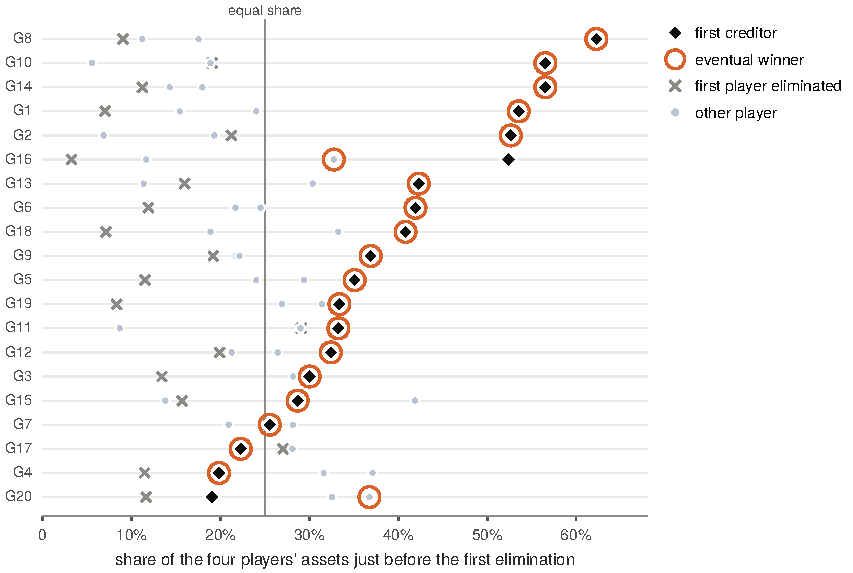
\includegraphics[width=0.86\linewidth]{fig_estates.pdf}
\caption{Each player's share of total assets at the first liquidation menu of the debt that ends in the game's first elimination. Assets are cash, deeds at list price (half if mortgaged) and buildings at cost. Games are ordered by the first creditor's share.}
\label{fig:estates}
\end{figure}

The other \fact{d.estate.discordant} games carry the information. In G4, G7, G15 and G17 the first creditor did not lead in assets and went on to win. In G20 it did not lead and lost. Where the creditor already led, it won \fact{d.estate.leader.creditorwins} of \fact{estate.first-creditor-leads-assets} games. G17 is the clearest case. Gemini declared bankruptcy on a \$550 rent with a payment route available, after telling the table that it was short.
\TranscriptQuote{g17-d234-public}
Its estate held six deeds, among them Park Place and Boardwalk with five houses. It went to Sol, which had the smallest asset share at the table and \$34 in cash, and Sol won. Five games cannot show that estates decide winners. They show that the first estate is more than a marker of who was already ahead.

Estates also end most of the stand-offs that bargaining does not. Of the \fact{barg.dyads.unsettled} pairs that never settled, the group was next completed through an estate in \fact{barg.dyads.unsettled-resolved-by-estate}, and \fact{barg.dyads.unsettled-resolved-by-nonterminal-estate} of those came before the game's last elimination. In \fact{barg.dyads.unsettled-same-completer-via-estate} the same would-be buyer received the group that way and paid nothing. A holder's refusal lasts only as long as the holder does. The agents in Incidents~\ref{inc:g1} and~\ref{inc:g13} bargain over exactly that, and the buyer in the last incident acts on it.

\IncidentTitle{g18}{A buyer stops buying once the seller needs the money (G18)}

At G18 turn 181 Opus holds \$615 and bids \$200 and then \$250 for Sol's mortgaged Pacific, which would complete Opus's greens. Sol holds \$294 and asks \$600.
\TranscriptQuote{g18-d420-note}
Sol rejects \$250. Over the next six turns Opus says four times that the offer still stands, the last time after collecting a \$750 rent from Sol.
\TranscriptQuote{g18-d431-assurance}
A second \$750 rent then forces Sol to sell its orange hotels and mortgage its reds, which leaves it \$49. Sol offers Pacific in a bundle for \$450 and then \$350 to pay for new orange houses, and Opus passes on both. Sol then names the price Opus had advertised.
\TranscriptQuote{g18-d441-invocation}
\TranscriptQuote{g18-d442-withdrawal}
\TranscriptQuote{g18-d442-explanation}
\IncidentOutcome{No sale occurs. Sol's note reads \InlineQuote{in-g18-d443-rebuild}. Opus, holding \$2,125, redeems its two green deeds over the next four turns and bids \$150 and \$225 for Pacific. Sol asks \$450, \$350 and \$300, and nothing settles. Sol is eliminated at turn 197, its estate passes to Opus, and Opus wins.}
\IncidentReading{While Sol had cash it priced the blocker at \$600. Down to \$49, it offered the same deed at the buyer's own price so that it could rebuild, and the buyer declined. Opus's returned explanation says that buying would only extend a nearly bankrupt rival's life, and as Sol's likely creditor it could expect the deed anyway. The assurance was a public message that the engine does not enforce, and nothing shows that it was insincere when made.}
\IncidentSource{G18 d419--d461. Sol's responses are standard first attempts. Opus's are action-only responses, and the explanation is the provider's reasoning field.}
